\documentclass[crop=false]{standalone}

\usepackage[subpreambles=false]{standalone}
\usepackage{import}
\usepackage{graphicx}
\usepackage{subcaption}
\usepackage{tikz}

\begin{document}


\begin{center}
  % \hspace*{-0.08\linewidth}
  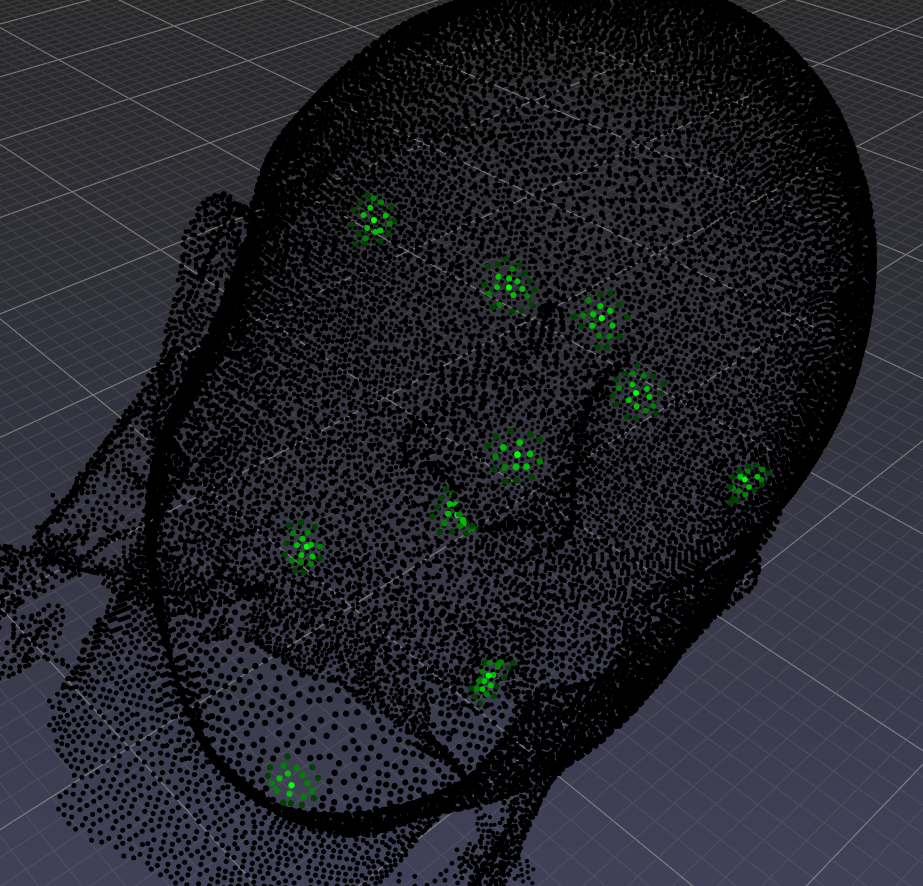
\includegraphics[width=\linewidth]{thesis/methods/import/imgs/gt_hs_clusters.png}
  %\vspace*{-0.06\linewidth}
  \captionof{figure}{
    \textbf{Prepared sample that serves as the ground truth input for the initial network.}
    \small The intensity of the green points represents the activation of each point. Activations are either 0 for background and 0.25, 0.5, 0.75 or 1 for points in landmark regions.
  }
  \label{fig:gt_hs_clusters}
\end{center}

\end{document}